% boosting.tex
% Jeremy Barnes, 29/8/1999
% $Id$

% The chapter of my thesis on Boosting

% commands.tex
% Jeremy Barnes, 1999
% $Id$

\providecommand{\emp}{\mathrm{emp}}
\providecommand{\calF}{\ensuremath{\mathcal{F}}}
\providecommand{\fat}{\ensuremath{\mathrm{fat}}}
\providecommand{\sign}{\ensuremath{\mathrm{sign}}}
\providecommand{\cop}{\ensuremath{\mathrm{co}_p}}
\providecommand{\co}{\ensuremath{\mathrm{co}}}
\providecommand{\bfx}{\ensuremath{\mathbf{x}}}
\providecommand{\bfy}{\ensuremath{\mathbf{y}}}
\providecommand{\bfyh}{\ensuremath{\hat{\mathbf{y}}}}
\providecommand{\calO}{\ensuremath{\mathcal{O}}}
\providecommand{\calI}{\ensuremath{\mathcal{I}}}
\providecommand{\calH}{\ensuremath{\mathcal{H}}}
\providecommand{\calX}{\ensuremath{\mathcal{X}}}
\providecommand{\ip}[2]{\ensuremath{\langle {#1} , {#2} \rangle}}
\providecommand{\lin}{\mathrm{lin}}
\providecommand{\calS}{\ensuremath{\mathcal{S}}}
\providecommand{\VCdim}{\mathrm{VCdim}}
\providecommand{\Fat}[1]{\mathrm{Fat}_{#1}}
\providecommand{\cover}[2]{\mathcal{N}({#1}, {#2})}
\providecommand{\covert}[3]{\mathcal{N}({#1}, {#2}, {#3})}
\providecommand{\MATLAB}{{\tt MATLAB}}
\providecommand{\C}{{\tt C}}
\providecommand{\argmin}{\mathrm{argmin}}

% Theorem-like constructs
\newtheorem{theorem}{Theorem}
\newtheorem{definition}{Definition}

\providecommand{\proof}{\par \par \noindent {\bf Proof:\ }}

\providecommand{\figlinewidth}{1pt}

\newenvironment{linefigure}%
		{\begin{figure} \rule{\textwidth}{\figlinewidth}}%
		{\rule{\textwidth}{\figlinewidth}\end{figure}}


\chapter{Boosting and similar algorithms}

The name ``Boosting'' is applied to many different machine learning
algorithms, which combine many weak hypotheses to form a ``strong''
hypothesis that significantly outperforms them.

This chapter will explore exactly what is meant by the term
``boosting'', including a formal definition.  The key features of
boosting are described, including the ``AdaBoost'' algorithm first
described by Freund and Schapire \cite{Freund96}.

A useful viewpoint of the boosting algorithm as an optimisation via
gradient descent in a cost space is then considered.  A result from
Mason et al. \cite{Mason99} is reproduced which shows that boosting is
indeed performing gradient descent.

We then turn to questions of the performance of boosted algorithms; in
particular guarantees on the training and generalisation error.
Several results are presented.

Finally, we consider \emph{normed boosting algorithms} where the
weights of the hypotheses are constrained by some norm.  Several
properties of these algorithms which are different from those of
unconstrained boosting algorithms are discussed.






\section{Definition of boosting}

In order to achieve a formal definition of boosting, we need the
following definitions.  This discussion follows \cite{Duffy99}.

Probably Approximately Correct



\section{AdaBoost}

AdaBoost is a machine learning algorithm
that combines many ``weak'' hypotheses to generate a hypothesis 
that usually performs significantly better than any of the weak
hypotheses.  Even the simplest of weak algorithms, when
``boosted'', will usually outperform the best unboosted algorithms.
\footnote{As a result, the focus of recent research effort has shifted from the
development of \emph{learning} algorithms (which are all more
or less equivalent when boosted) to the development of better \emph{boosting}
algorithms.}

These weak hypotheses are combined in a linear combination.
The weight of each weak hypothesis (the
\emph{classifier weight}) depends upon the performance of that
classifier on the training dataset.  Section \ref{sec:classifier
weights} describes these classifier weights in more detail.

Each sample in the training dataset is given a weight (\emph{sample
weight}) which is modified depending upon how ``hard'' that
sample is to classify.  Section \ref{sec:sample weights} describes
these sample weights in more detail.

A more thorough description of boosting is given in appendix
\ref{chapter:boosting details} and \cite{Freund96}.

\subsection{Classifier weights}
\label{sec:classifier weights}

The AdaBoost algorithm combines a number of ``weak'' classifiers
$f_1(\cdot), \ldots, f_n(\cdot)$ in a linear combination to produce a
``stronger'' classifier $F(\cdot) = \sum_{i=1}^{n} b_i f_i(\cdot)$.
The coefficients $b_i$ are subject to the condition that they produce a
convex combination where $\|b\|_1 = \sum_{i=1}^{t} b_i = 1$.

AdaBoost's training process is divided into iterations.  On iteration
$t$, one weak learner $f_t(\cdot)$ is added to the linear
combination ($f_t$ is chosen by the weak learning algorithm).  The
coefficient $b_t$ of $f_t$ is calculated from the 
training error $\epsilon_t$ of $f_t$ as 
%
\begin{equation}
b_t = - \log \frac{\epsilon_t}{1 - \epsilon_t}
\label{eqn:theory:bt}
\end{equation}
%
When $\epsilon_t = 1/2$, the classifier only does as
well as random guessing, and has $b_t = 0$.  As
$\epsilon_t$ approaches zero, $b_t$ increases without bound.  The
effect is that $F$ becomes dominated by those weak hypotheses that
performed well on the training samples
\footnote{Training is halted if $\epsilon_t = 0$ or $\epsilon_t \geq 1/2$.}.  The weights are normalised once training is completed.


\subsection{Sample weights}
\label{sec:sample weights}

Each sample in the training set has a corresponding weight $w_j$ which
is updated to reflect the difficulty of that sample.  On each iteration the
weights of samples which $f_t$ classified incorrectly are increased
(scaled by $\exp \{ -b_t \}$); the whole lot are then normalised.
This function has the following effect on distribution of weights:

\begin{itemize}

\item	Training samples which are misclassified often, or are one of 
	few points to get misclassified, increase their proportion of
	the weight (are identified as ``hard samples'');

\item	Other samples decrease their proportion of the weight, and are
	identified as ``easy'' samples.

\end{itemize}

The overall effect is for those samples near the decision boundary to
increase in weight, and those far from it to decrease.  This forces
the algorithm to concentrate on the hard samples, and is one reason
why it works well on low-noise datasets.  Unfortunately, those samples
corrupted by noise are usually hard also, and concentrating on those
is not desirable.

\section{AdaBoost}
\label{sec:adaboost}

This section provides an explicit and detailed description of the
boosting algorithm as a complement to the implicit description in
chapter \ref{chapter:theory}.

\par

\noindent{\bf Input:} $l$ examples $(\bfx_1, \bfy_1), \ldots, (\bfx_l,
\bfy_l)$
\par
\noindent{\bf Initialisation:} $w_i|_{t=1} = 1/l$ for $i=1 \ldots l$
\par
\noindent {\bf Do for} $t=1 \ldots T$:


\begin{enumerate}

\item	Train weak learner on the weighted sample set 
	$(\bfx_1, \bfy_1, w_1) \ldots (\bfx_l, \bfy_l, w_l)$
	and obtain weak learner $f_t(\cdot) : \calI \mapsto \{\pm 1\}$

\item	Calculate the training error $\epsilon_t$ of $f_t(\cdot)$:
	%
	\begin{equation}
	\epsilon_t = \sum_{j=1}^l w_j |_t 
	I \left( f_t(\bfx_j) \neq \bfy_j\right)
	\end{equation}

	If $\epsilon_t = 0$ (a single weak learner can correctly learn
	the relationship) or $\epsilon_t \geq \phi - \Delta$ (where
	$\Delta$ is a small positive constant; thus the weak
	learner is performing as badly as random guessing) then abort
	the training process.

\item	Calculate our classifier weight $b_t$:
	\begin{equation}
	b_t = \log \frac{\epsilon_t}{1 - \epsilon_t}
	\end{equation}

\item	Update the weights $w_i$:
	%
	\begin{equation}
	w_i|_{t+1} = \left\{
	\begin{array}{cl}
		w_i|_t / Z_t	&	\qquad \qquad \mbox{if
		$f_t(x_i) = y_i$} \\
		w_i|_t / Z_t \exp \left\{ -b_t \right\} & \qquad \qquad
		\mbox{otherwise} \\
	\end{array} \right.
	\end{equation}

	where $Z_t$ is a normalisation constant, such that
	$\sum_{i=1}^{l} w_i|_{t+1} = 1$
\end{enumerate}

\par
\noindent {\bf Output:} 
\begin{equation}
F'(\bfx) = \sign \left\{ \sum_{i=1}^T w_i f_i(\bfx) \right\}
\end{equation}


\section{Boosting as gradient descent}
\label{sec:theory:gradient descent}

Recent work has shown boosting to be an implementation of gradient
descent in an inner product space \cite{Mason99}\footnote{This
discussion follows Mason et al. \cite{Mason99} rather closely with
some changes in notation and omission of details such as stopping
criteria.}.
An inner product space requires both a universal set
$\mathcal{X}$ and an inner product operator \ip{\cdot}{\cdot}.  We
define
%
\begin{equation}
\calX = 
\mathrm{co} (\calF) \doteq
 \bigcup _{n \in \mathbb{N}}
\left\{
 \sum_{i=1}^{n}
  b_i
f_i : f_1, \ldots, f_n \in \calF,
 b_1, \ldots, b_n \in \mathbb{R},
 \sum_{i=1}^{n} | b_i | = 1
\right\} \cup \emptyset
\end{equation}
%
(which is the convex hull of \calF), and
%
\begin{equation}
\ip{F}{G} = \frac{1}{l} \sum_{i=1}^{l} F(\bfx_i)G(\bfx_i) \qquad
F, G \in \calX
\end{equation}
%
We also choose the cost function
%
\begin{equation}
C(F) = \frac{1}{l} \sum_{i=1}^{l} \exp
\left\{ -y_i F(\bfx_i) \right\}
\label{eqn:theory:cost function}
\end{equation}

At iteration $t$ of gradient descent, we wish to choose a function $f_t$ and
a weight $b_t$ such that $C(F + b_t f_t)$ decreases (the choice of
$f_t$ is made indirectly through the choice of the sample weights
$w|_t$).  In other words, we are asking for sample weights $w|_t$ that
choose a \emph{direction} $f_t \in \calF$ such that $C(F + b_t f_t)$
decreases as fast as possible.  This direction is the negative of the
functional derivative of $C$:
%
\begin{equation}
f = -\nabla C(F)(\bfx) = \left. \frac{\partial C(F + \alpha
1_{\bfx})}{\partial \alpha} \right|_{\alpha = 0}
\label{eqn:functional derivative}
\end{equation}
%
where $1_{\bfx}$ is the indicator function of $\bfx$; this is
necessary as we can only evaluate \ref{eqn:functional derivative} at
points where we have a sample.  Since the
optimal $f_t$ will not necessarily be in $\calF$, we choose the
$f \in \calF$ with the greatest inner product $\ip{-\nabla
C(F)}{f}$.

Having chosen our direction, we now choose a step size $b_t$.
AdaBoost uses a line search for the minimum of the cost functional
along this line
%
\begin{equation}
b_t = \arg \min_{b_t} \sum_{i=1}^{l} C(y_i F(\bfx_i) + y_i b_t f_t(\bfx_i)
\end{equation}
%
which (for the cost function (\ref{eqn:theory:cost
function})) has a closed-form solution  (\ref{eqn:theory:bt}).  Thus, the
boosting algorithm implements gradient descent.  The process is
illustrated in figure \ref{fig:gradient descent}.

\begin{figure}
\begin{center}
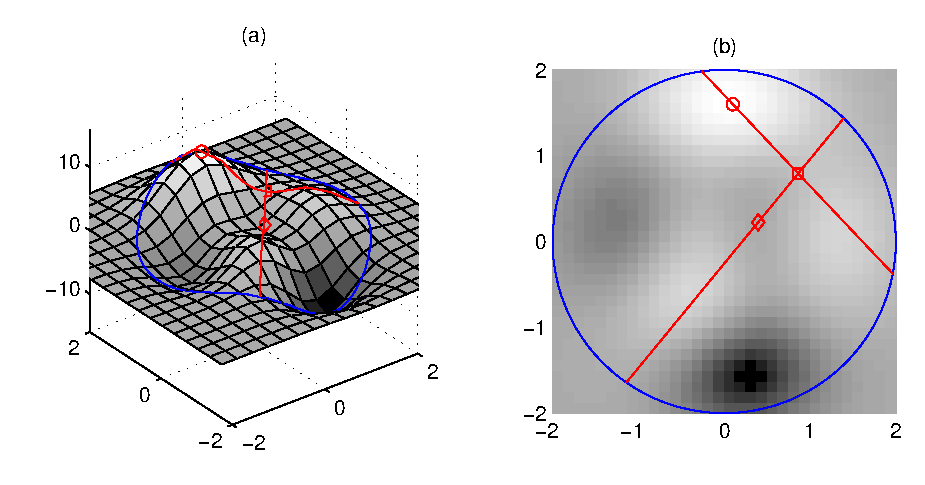
\includegraphics{figures/descent.epsg}
\caption{Schematic representation of gradient descent.  Points within the blue
circle are in \calF, the height of the surface the value of
(\ref{eqn:theory:cost function}) at that point.  (a) is a 3D view, (b)
is top view. Red lines show line searches; markers minimums.  Descent
from $\circ$ to $\Box$ to $\Diamond$, where it terminates due to
local minimum.}
\label{fig:gradient descent}
\end{center}
\end{figure}


\section{Normed boosting algorithms}

\section{Performance evaluation}


\subsection{Convergence of boosting}
Theorem: Given a weaklearner $\mathcal{L}$ and a training set $S$,
then either:
\begin{enumerate}
\item	The boosting algorithm will terminate; or
\item	There exists an iteration $t_{zero}$ such that for all $t \geq
	t_{zero}$ the training error $\epsilon_t = 0$.
\end{enumerate}
If for any training iteration $t$ we have $\epsilon_t > 1/2$ then the
boosting algorithm will terminate.  Assuming that this is not the
case, let us look at $\|b\|$.  As $t \rightarrow \infty$, $\|b\|
\rightarrow \infty$.  Thus, taking the normalised hypotheses $\bar{h}_i
= b_i \frac{h}{\sum b}$ we get the cost function as
\[
C(F_{t+1}) = \sum_{i=1}^{m} \exp\left\{ -y_i b_i h_i(x_i)
\right\}^{\|b\|}
\]
Now, we know from theorem (number?) that the boosting algorithm will
always find the global minimum of the cost function.  Since all $b_i >
0$, this is achieved when all training examples are classified
correctly...

Need a lot more work on this proof.  Do I want to show that since it
gets steeper and steeper, the cost of a negative sample gets too
large?  I don't think that the way I am doing it is going to work,
really.  I need to show that because
\begin{itemize}
\item	The weights for wrong samples are increasing exponentially,
	and
\item	The power that the cost function is raised to makes the wrong
	margin get worse and worse,
\end{itemize}
then the thingy gets minimised...

I need to bring the training error < 1/2 into it somewhere.  I think
that I can show that if
\begin{itemize}
\item	$\|b\|$ increases without bound; and
\item	$\epsilon_t$ is always < 1/2, then
\end{itemize}
I don't know!




\subsection{Size of $b$}
Theorem: The size of the $b$ weight vector, $\|b\| \rightarrow \infty$
as $t \rightarrow \infty$ (assuming the boosting algorithm doesn't
terminate).

Proof: ?


\subsection{Minimum margin}
Theorem: Given a particular learning algorithm $F$ and a training
set $S$, then define the minimum margin as
\[
m_{\min} = min_{\{x,y\} \in S} y_i F(x_i)
\]
Then the boosting algorithm will converge as $t \rightarrow \infty$ to
the solution which maximised the minimum margin.

Proof: For boosting we can write $F_t = b_1 f_1 + \cdots + b_t f_t$.
Then defining our \emph{normalised hypotheses} $\bar{f}_i$ as
\[
\bar{f} = \frac{b_i f_i}{\|b\|}
\]
such that $\hat{F}_t = \bar{f}_1 + \cdots + \bar{f}_t$, we can write
our cost function (reference?) as 
\[
C(b, S) = \sum_{i=1}^{m} \exp\{-y_i \bar{F}_t(x_i)\}^{\|b\|}
\]
We already know from the gradient descent theory (reference?) that we
are trying to minimise the cost function.  Now as $\|b\| \rightarrow
\infty$ (from the previous theorem) the largest value of $\exp\{-y_i
\bar{F}_t(x_i)\}$ will dominate, and so $C(b, S) \rightarrow exp\{\max
-y_i \bar{F}_t(x_i)\}$.  Thus, by minimising $C(b, S)$, we are making
$\min y_i \bar{F}_t(x_i)$ as large as possible; that is we are
maximising the minimum margin.
